\documentclass[]{article}

\usepackage[english]{babel}
\usepackage[utf8x]{inputenc}
\usepackage[T1]{fontenc}
 
\usepackage[a4paper,margin=2 cm]{geometry}
 
%% Useful packages
\usepackage{amsmath}
\usepackage{graphicx}
\usepackage{para list}
\usepackage{indentfirst}
\usepackage{booktabs}
\usepackage{multirow}
\usepackage{clrscode}
\usepackage{listings}
\usepackage{multicol}
\usepackage{graphicx}

\begin{document}
\title{Experiments Report of Automatic Speech Recognition }
\author{s1626868   s1469487}
\maketitle
\begin{multicols*}{2}

\section{Introduction}

In this experiment, we apply different methods to continuous word recognition on the TIMIT speech data set using the Kaldi automatic speech recognition toolkit. We will first do experiments about 4 aspects of monophone model. They are number of Gaussian, different features, dynamic features and CMN/CVN. Then, we will move on to triphone model to investigate how the number of cluster and Gaussian influence the performance. Finally, we will try to build a gender dependent recognition system and using different adaptive methods to our baseline model.

\section{Monophone Model}
\subsection{Number of Gaussian}
\subsubsection{Purpose}
The aim of this task is to investigate how the number of Gaussian mixture components influences WER, and find the optimal number that gives the lowest WER. 

\subsubsection{Implementation}
We want to test the model with different number of Gaussian mixture components. So, we modify the parameter of $train\_mono.sh$ script.

\begin{lstlisting}[language=sh,showstringspaces=false,numbers=left,tabsize=4, xleftmargin=\parindent, frame=single, basicstyle=\tiny] 
# we previously set a parameter $num_gauss to
# store the number of gaussian 
steps/train_mono.sh --nj 4 --totgauss $num_gauss \
	data/train data/lang exp/mono
\end{lstlisting}

To evaluate the time consuming, we also compute the the time used in the process of training model and decoding.

\begin{lstlisting}[language=sh,showstringspaces=false,numbers=left,tabsize=4, xleftmargin=\parindent, frame=single, basicstyle=\tiny] 
# store start time
start_time=$(date +%s)

# code to train model and decode
......

# store end time
end_time=$(date +%s)

# compute runing time
echo "runing time" $(($end_time - $start_time))

\end{lstlisting}

scripts: \textbf{\\ \indent exp\_mono\_t1.sh  \\ \indent run\_mono\_t1\_best.sh}

\subsubsection{Experiments and Results}
We start with setting a large range for the number of Gaussian mixture components (n), starting from 500  and going till 20000 with the step of 250. The results of the experiment in terms of WER and time are shown in Figure 2.1.1 and Figure 2.1.2 respectively.

\begin{center}
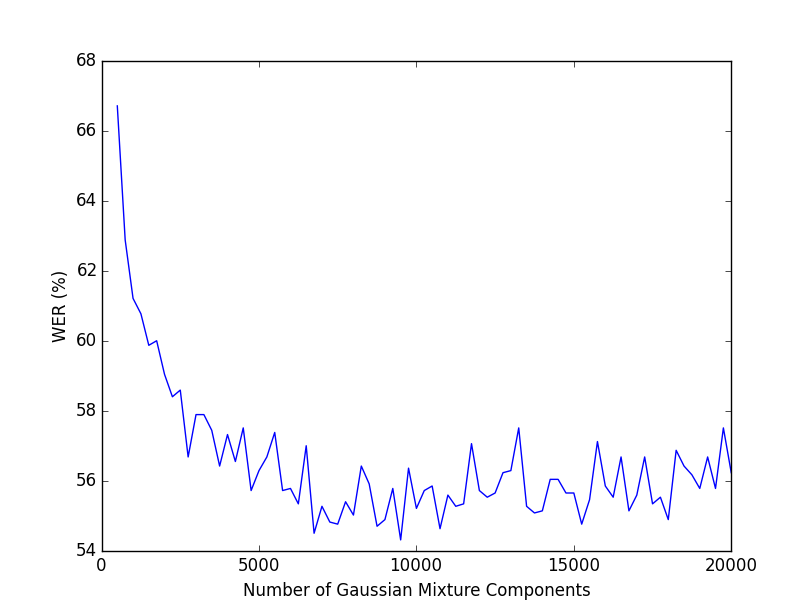
\includegraphics[width=3in]{figure_1_WER.png} 
Figure 2.1.1: WER against number of Gaussian mixture components (500<n<20000).
\end{center}

\begin{center}
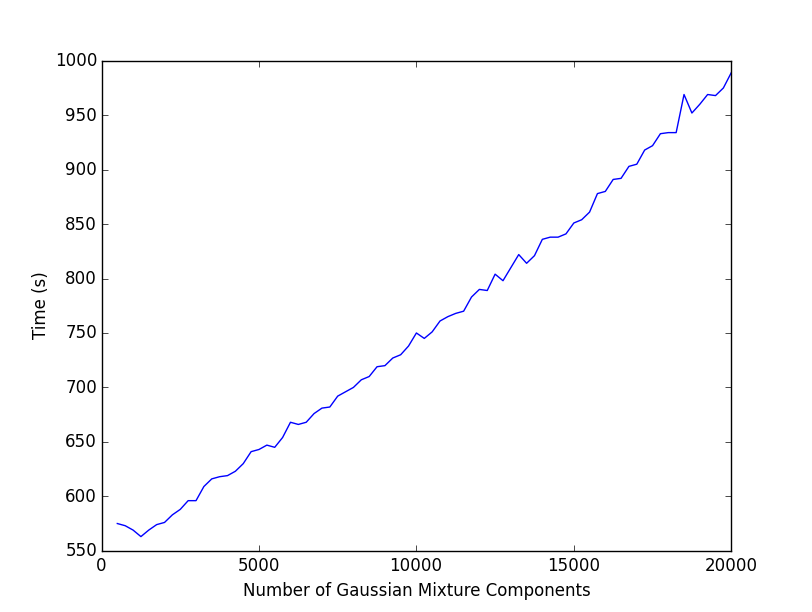
\includegraphics[width=3in]{figure_1.png} 
Figure 2.1.2: Time against number of Gaussian mixture components (500<n<20000).
\end{center}

As we can see from Figure 1.1.2, the time consuming increases linearly with the increase of the number of gaussian mixture components.  According to Figure 1.1.1, WER generally decreases with the increase of Gaussian mixture components when n<10000. After that, WER tends to convergence, fluctuating between 54\% and 58\%. The lowest WER occurs around n=9500, so we focus on the range (9500,9800) to run our script again in order to see if we could generate a better result in that range. Figure 1.1.3 shows the result of further experiment.
\begin{center}
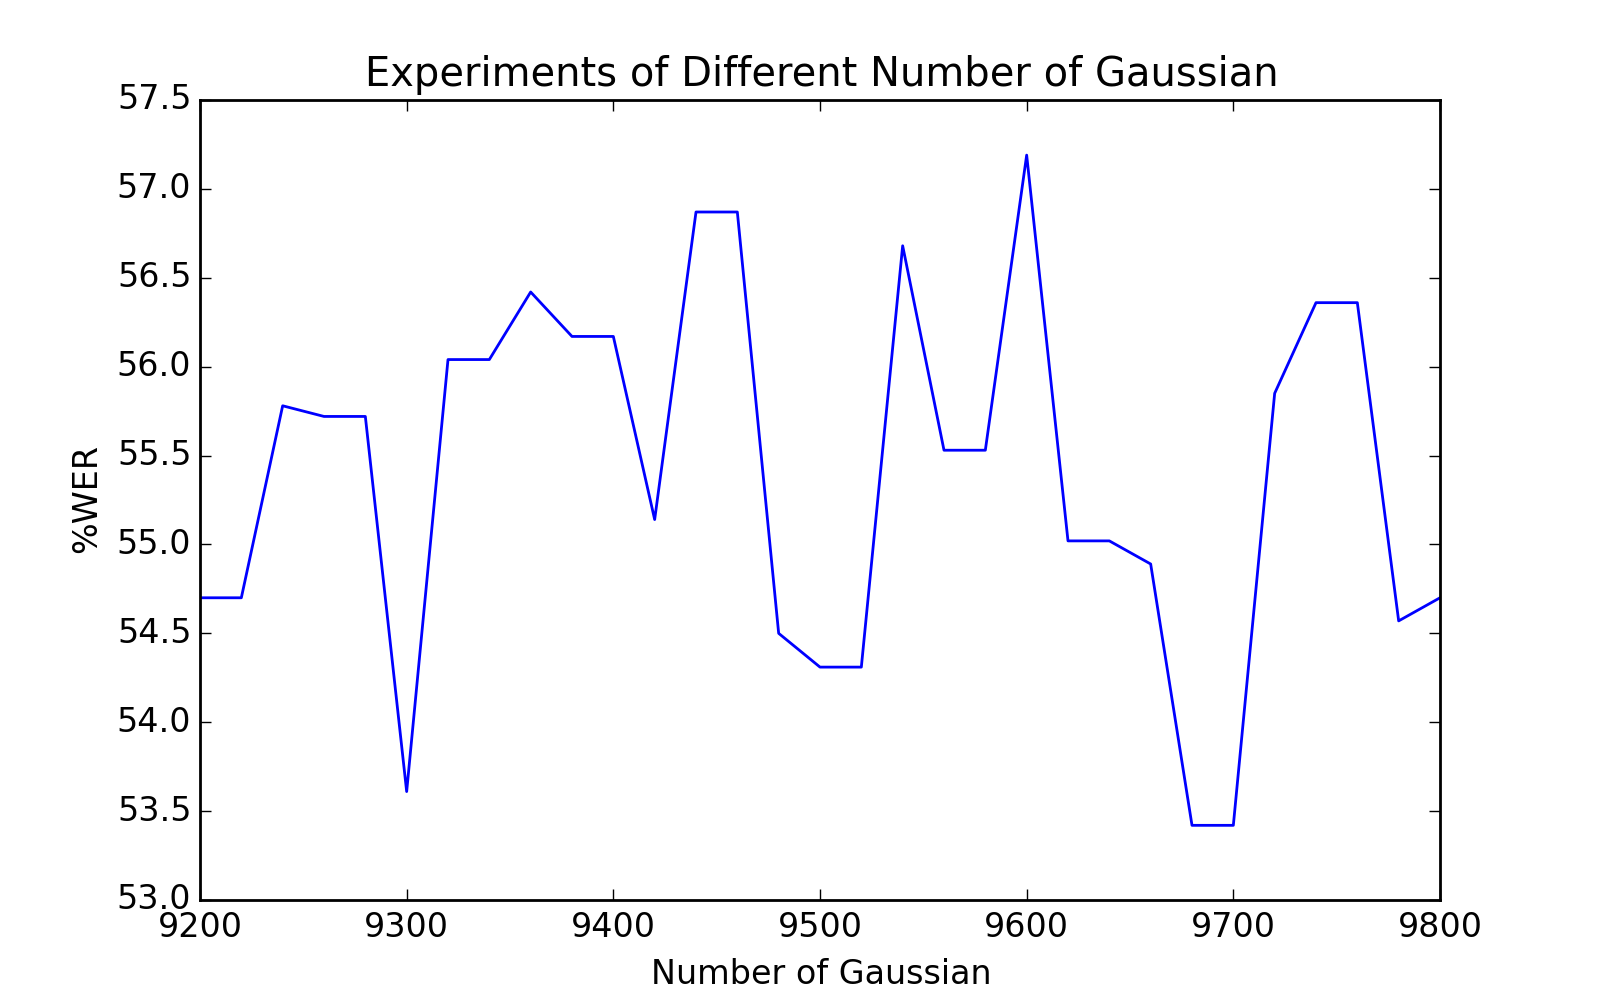
\includegraphics[width=3in]{result1_detailed_wer_new.png} 
Figure 1.1.3: WER against number of gaussian mixture components (9500<n<9800).
\end{center}
Form the plot, we find that the lowest WER we obtained is 53.42\%  , where the number of gaussian mixture components is about 9700.

\subsubsection{Conclusion and Discussion}
From the results we got in experiments, we could investigate that with the increase of the number of gaussian mixture components, the WER decreases on the whole. When the number of gaussian is less than 3000, the WER decreases smoothly. After that, the evolution of WER starts fluctuating but still has the trend of decreasing. Until the number of gaussian mixture components reaches around 7000, the WER fluctuates in a small range. So, to sum up, the WER will finally converge with the increase of number of gaussian mixture components.

To briefly explain this, we refer to Mark's review work. We think if we give a large number of gaussian, the gaussians used to express the distribution of state transformation of each phone increases so that the distribution is characterized very precise. This is the reason why a higher gaussian will lead to a better recognition result. Meanwhile, too much gaussian will also cause some problem because the extra components will cause noise as well. This explains the cause of fluctuating parts of the evolution plot.

As for the time consuming, we could easily come to this conclusion that the time consuming has a perfect linear relationship with the number of gaussian mixture components. So, to search the best model, we could try small gaussians to save time.

The best model we obtained is shown in script run\_mono\_t1\_best.sh (where the number of gaussian mixture components is 9700).

\subsection{Features}
\subsubsection{Purpose}
The aim of this part is to use MFCC, PLP and Filter bank with the optimal number of Gaussian mixture components(9700) obtained in task 1.1 to investigate how different acoustic features give different WERs. 

\subsubsection{Implementation}
To extract different kinds of features(mfcc, plp and fbank), we write a loop in script to obtain different features.

\begin{lstlisting}[language=sh,showstringspaces=false,numbers=left,tabsize=4, xleftmargin=\parindent, frame=single, basicstyle=\tiny] 
for feats in mfcc plp fbank; do
	for dir in train test; do
		# extract features
		steps/make_$feats.sh data/$dir /
			exp/make_$feats/$dir $feats
		# compute cmvn
		steps/compute_cmvn_stats.sh data/$dir /
			exp/cmvn/$dir cmvn
	done	
	# code to train model and decode
	......
done

\end{lstlisting}

scripts: \textbf{\\ \indent exp\_mono\_t2.sh}

\subsubsection{Experiments and Result}
Figure 2.2.1 and Figure 2.2.2 respectively show the comparisons among the three acoustic features in terms of WER and time.

\begin{center}
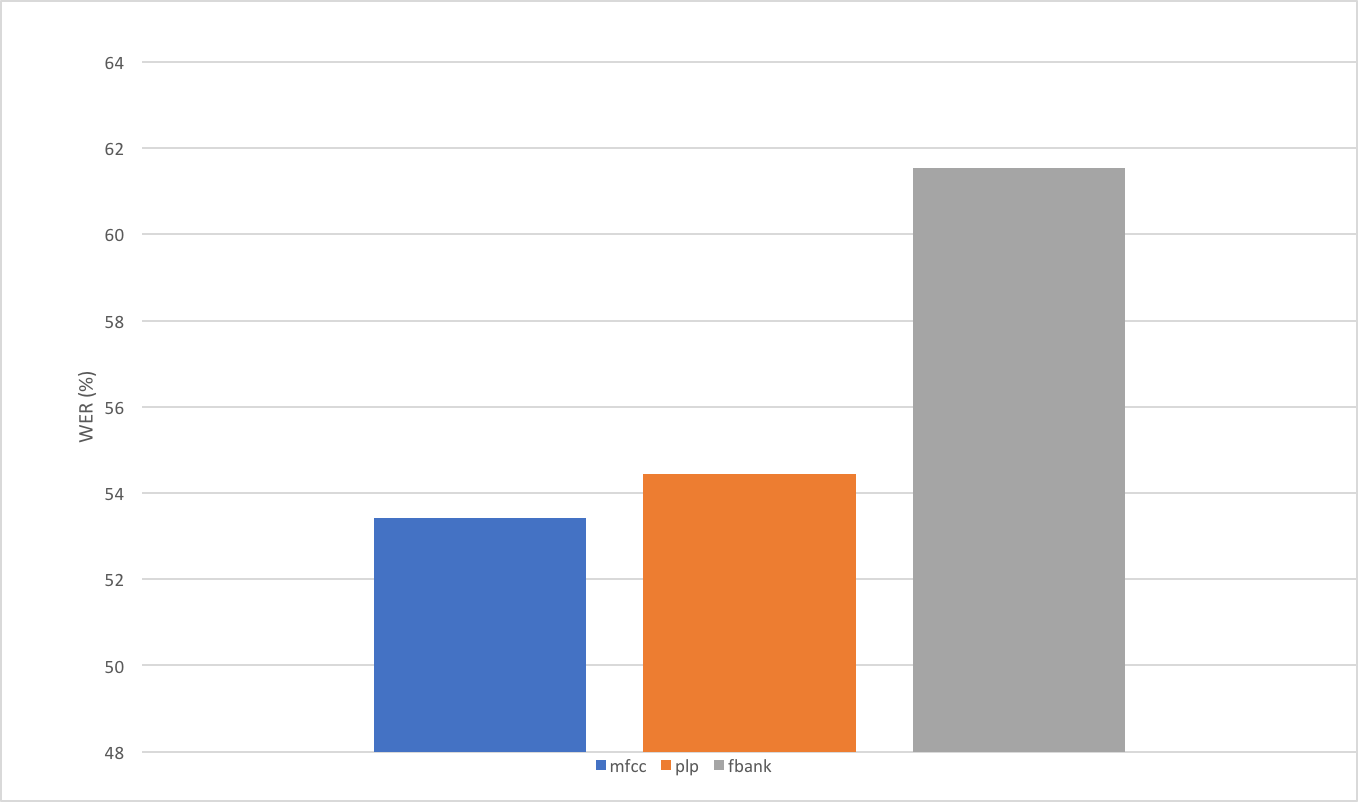
\includegraphics[width=3in]{Picture2.png} 
Figure 2.2.1: WERs of different acoustic features.
\end{center}

\begin{center}
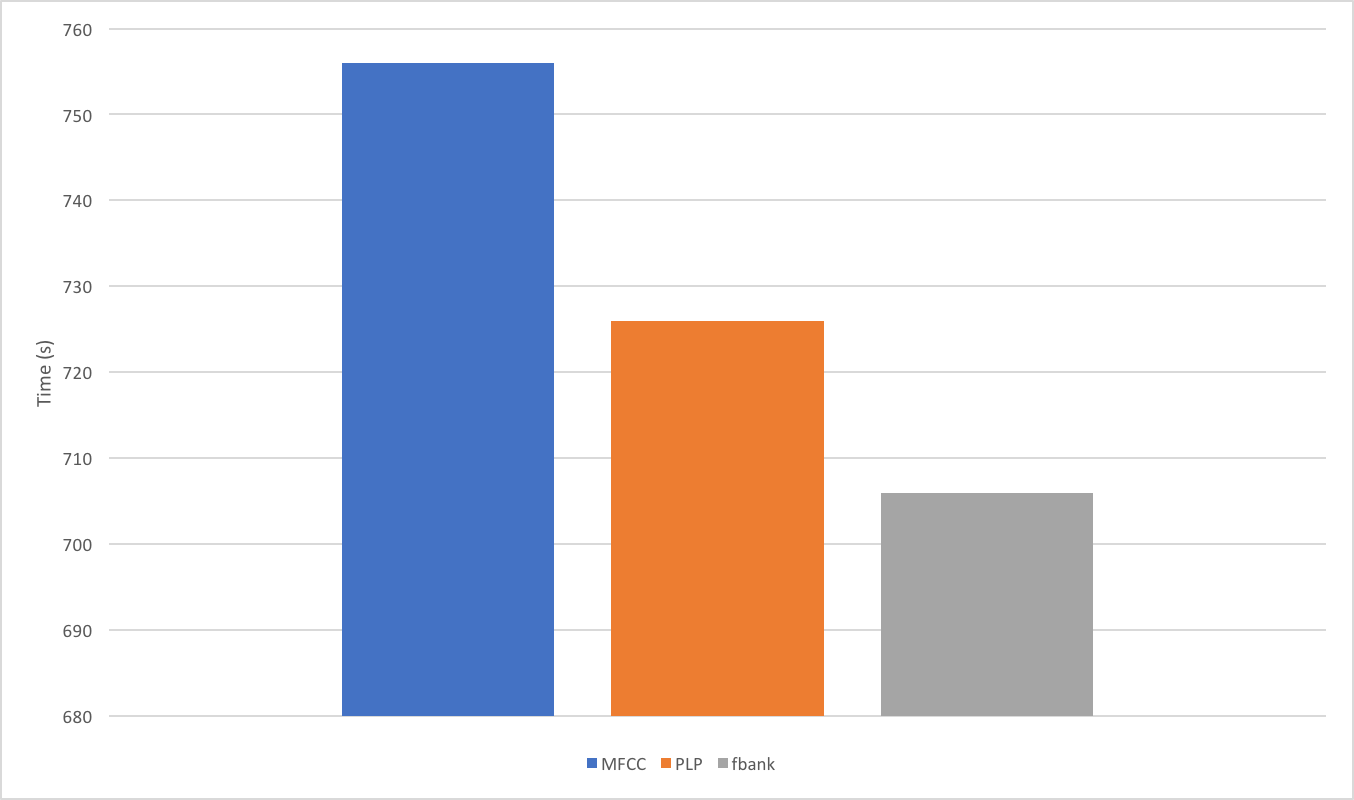
\includegraphics[width=3in]{Picture1.png} 
Figure 2.2.2: Time of different acoustic features.
\end{center}

WERs of MFCC, PLP and Fbank are 53.42\%, 54.44\% and 61.53\% respectively. Time of MFCC, PLP and Fbank are 756s, 726s and 702s respectively. MFCC has the lowest WER while the WER of Fbank is much higher than that of MFCC and PLP. However, Fbank takes the shortest time, PLP is the second and MFCC needs the longest time.

\subsubsection{Conclusion and Discussion}

MFCCs are based on the log spectral envelope of the speech signal, transformed to a nonlinear frequency scale that roughly corresponds to that observed in the human auditory system.This kind of feature is widely used in standard HMM-GMM model. However, it's not robust against noise.

Perceptual linear prediction(PLP) feature uses linear predictive auto-regressive modelling to obtain cepstral coefficients. it is a frequently used alternative acoustic feature analysis, which  includes an auditory-inspired cube-root compression and uses an all-pole model to smooth the spectrum before the cepstral coefficients are computed (Hermansky, 1990). And it is better noise robustness.

As for Fbanks, it is a part of MFCCs features and is widely used in DNN ASR model.

As what is shown in the plot, MFCCs and PLP could obtain similar results and Fbank gives the worst result though it costs less time. Therefore, in conclusion, MFCCs and PLP are very good features in automatic speech recognition task.

So, what advantages do MFCCs and PLP have? A particular advantage of cepstral representations compared with spectral representations is the decorrelation of cepstral  coefficients,  compared  with  the  high  correlations  observed  between neighbouring spectral coefficients(R\&H review, 2010). Such decorrelations are very well matched with the distributional assumptions that underlie systems based on Gaussians with diagonal covariance matrices.

\subsection{Dynamic Features}
\subsubsection{Purpose}
The aim of this task is to investigate how the dynamic features (i.e. delta and delta delta features) of MFCCs influence WER. To generate comparable result, we set the $--use-energy$ to false for all MFCCs in this experiment.

\subsubsection{Implementation}
The scripts use the pipeline to generate the dynamic features of the extracted features. 

The original code of generating features is:

\begin{lstlisting}[language=sh,showstringspaces=false,numbers=left, title=\lstname{Creating dynamic feature with pipeline method},tabsize=4, xleftmargin=\parindent, basicstyle=\tiny, frame=single] 
feats="ark,s,cs:apply-cmvn $cmvn_opts \
	--utt2spk=ark:$sdata/JOB/utt2spk \
	scp:$sdata/JOB/cmvn.scp \
	scp:$sdata/JOB/feats.scp ark:- | \ 
	add-deltas $delta_opts ark:- ark:- |";;
\end{lstlisting} 

We find that the dynamic features(delta and delta-delta features) are generated in third line with $add-delta$ command. So, we delete this part for not creating dynamic features. New code is shown below:

\begin{lstlisting}[language=sh,showstringspaces=false,numbers=left, tabsize=4, xleftmargin=\parindent, basicstyle=\tiny, frame=single] 
feats="ark,s,cs:apply-cmvn $cmvn_opts \
	--utt2spk=ark:$sdata/JOB/utt2spk \
	scp:$sdata/JOB/cmvn.scp \
	scp:$sdata/JOB/feats.scp ark:- |";;
\end{lstlisting} 

To obtain delta feature, we could simple option $--delta-order=1$ in $add-delta$ command. 

To check the new features without dynamic feature, we display the dimension of new features by using below command:

\begin{lstlisting}[language=sh,showstringspaces=false,numbers=left,tabsize=4, xleftmargin=\parindent, frame=single, basicstyle=\tiny] 
apply-cmvn --utt2spk=ark:data/train/utt2spk \ 
	scp:data/train/cmvn.scp \
	scp:data/train/feats.scp ark:- | \
	feat-to-dim ark:- -
	
# output:
13
\end{lstlisting}

scripts: \textbf{\\ \indent exp\_mono\_t3.sh}


\subsubsection{Experiment and Result}
We set the number of Gaussian mixture components to be 9700. Since the sample scripts used in the labs employ dynamic features, we copied train\_mono.sh and decode.sh to my-local and deleted the delta features in the codes. The original method using delta and delta-delta features obtains a WER of 53.42\%. The method using only delta feature obtains a WER of 60.51\% while the method using no dynamic feature obtains a WER of 81.34\%. The results of this experiment is shown in Figure 1.3.1 and Figure 1.3.2. 

\begin{center}
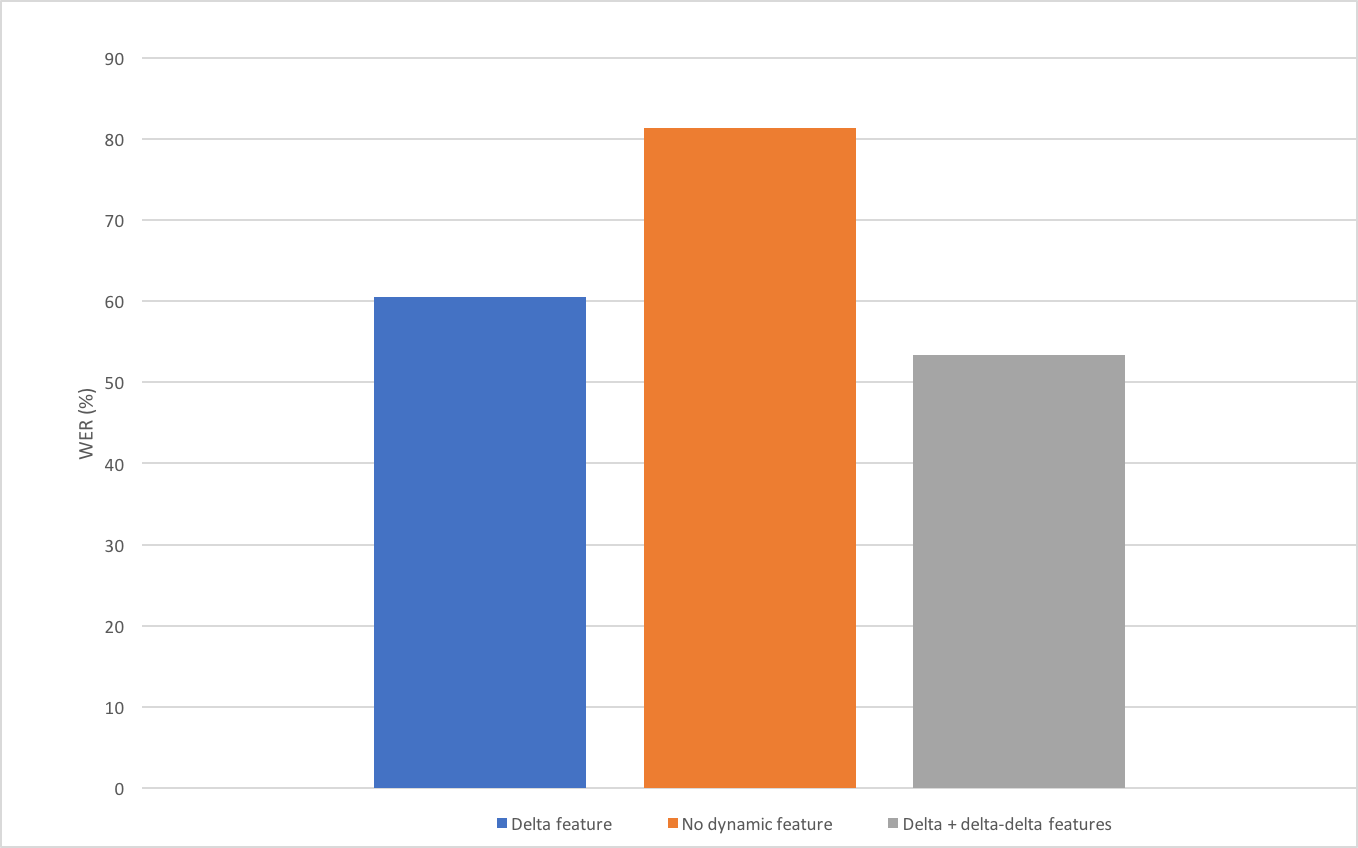
\includegraphics[width=3in]{Picture4.png} 
Figure 2.3.1: WERs of using and not using dynamic features.
\end{center}

\begin{center}
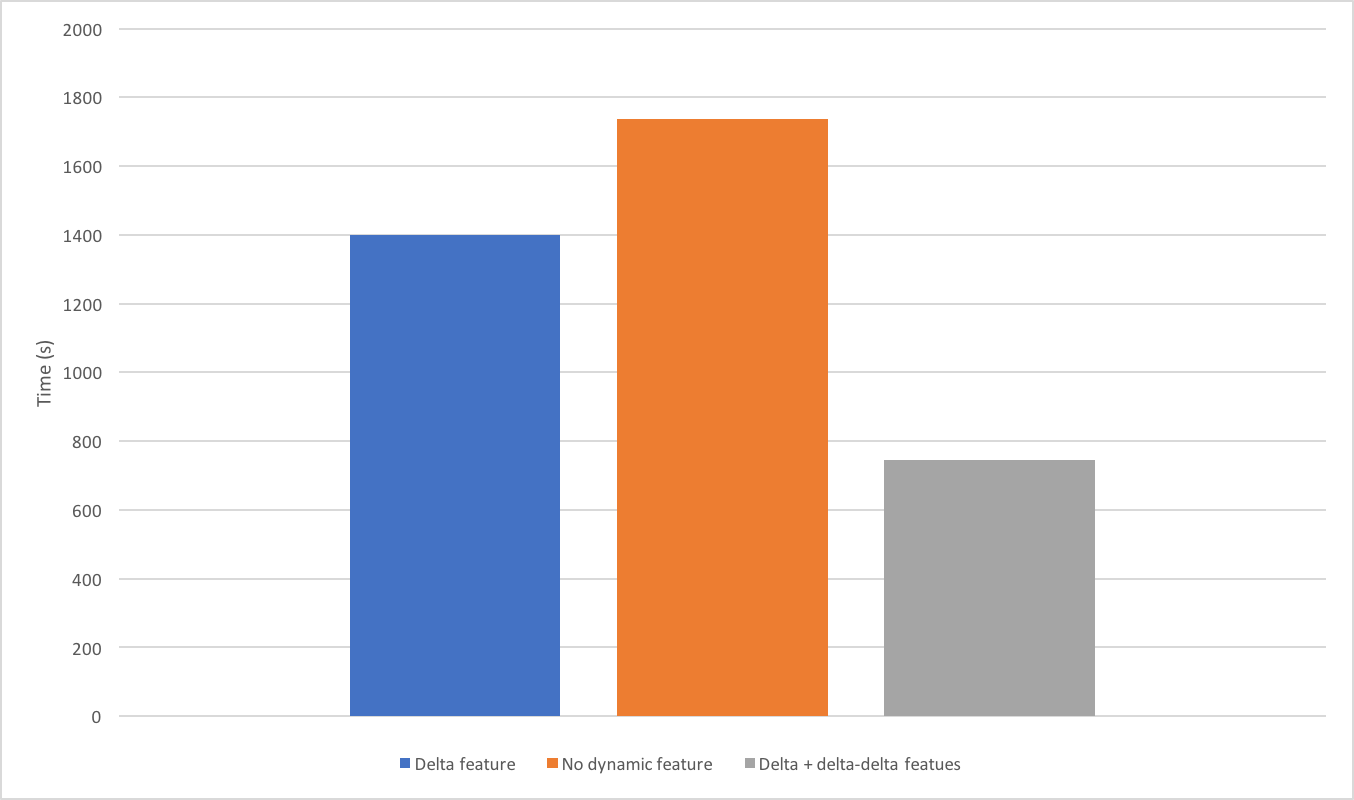
\includegraphics[width=3in]{Picture3.png} 
Figure 2.3.2: Time of using and not using dynamic features.
\end{center}

We can see that using delta feature and delta-delta feature (dynamic features) can much decrease the WER and time.

\subsubsection{Conclusion and Discussion}
From the experiment results, we could find that dynamic feature significantly improves the recognition result. The dynamic feature is generated by adding features to do with how the cepstral coefficients change over time. Speech recognition accuracy is substantially improved if the feature vectors are augmented with the first and second temporal derivatives of the acoustic features (sometimes referred to as the deltas and delta-deltas), thus adding some information about the local temporal dynamics of the speech signal to the feature representation (Furui, 1986)

Adding such temporal information to the acoustic feature vector introduces a direct dependence between successive feature vectors, which is not usually taken account of in acoustic modelling; a mathematically correct treatment of these dependences has an impact on how the acoustic model is normalized—since fewer feature vector sequences will be consistent—and results in an approach we may be viewed as modelling an entire trajectory of feature vectors.

\subsection{CMN/CVN}
\subsubsection{Purpose}
The aim of this task is to investigate the influence of CMVN on WER. In the sample scripts, CMVN is used. So, we avoided using CMVN in the experiment.
\subsubsection{Implementation}
We find that there is a parameter in $compute\_cmvn\_stats.sh$ that could help to create the features without CMVN, which is the $fake$ option. So, we modify the extracting feature part like this.
\begin{lstlisting}[language=sh,showstringspaces=false,numbers=left,tabsize=4, xleftmargin=\parindent, frame=single, basicstyle=\tiny] 
for dir in train test; do
	# extract features
	steps/make_mfcc.sh data/$dir /
		exp/make_mfcc/$dir mfcc
	# compute fake cmvn
	steps/compute_cmvn_stats.sh --fake data/$dir /
		exp/cmvn/$dir cmvn
\end{lstlisting}

scripts: \textbf{\\ \indent exp\_mono\_t4.sh}

\subsubsection{Experiment and Result}
We set the number of Gaussian mixture components to be 9700. The WER we got without using CMVN is 58.40\%, higher than 53.42\% (using CMVN). However, the time of using no CMVN is 736s whcih is 20s  shorter than that of using CMVN.

\subsubsection{Conclusion and Discussion}

Cepstral mean and variance normalisation (CMN/CVN) is a commonly applied technique which involves normalising the feature vectors, on a component-by-component basis, to zero mean and unit variance.(R\&H review,2010)

Cepstral mean normalisation (CMN) removes the average feature value
of the feature-vector from each observation. And cepstral variance normalisation (CVN) scales each individual feature coefficient to have a unit variance.

CMN/CVN could improve the recognition accuracy because it makes the feature robust to linear filtering such as that arising from varying type or position of microphones, or characteristics of a telephone channel.

Therefore, generally speaking, CMN/CVN reduce feature sensitive to the noise. 

\section{Triphone Model}
\subsection{Purpose}
The aim of this task is to investigate the influences of the number of clusters and the number of Gaussian mixture components on WER and seek a optimal com- bination that gives the lowest WER.
\subsection{Implementation}
This time, we want to investigate two parameters of $train\_deltas.sh$ script in exponential range. So, the experiment script is modified like this.
\begin{lstlisting}[language=sh,showstringspaces=false,numbers=left,tabsize=4, xleftmargin=\parindent, frame=single, basicstyle=\tiny] 
for ((num_cluster=1000;num_cluster<=4000; \
	num_cluster=um_cluster+1000)); do
	for ((per_gauss=1;per_gauss<=64; \
		per_gauss=per_gauss*2)); do
		# code to train model and decode
		......
	done
done
\end{lstlisting}

scripts: \textbf{\\ \indent exp\_tri\_t1.sh  \\ \indent run\_tri\_t1\_best.sh}

\subsection{Experiment}
We set the number of clusters to start from 2500 to 10000, with the steps of 500. The number of Gaussian mixture components starts from 15000 to 30000 in steps of 5000. The results are shown in Figure 2.

\begin{center}
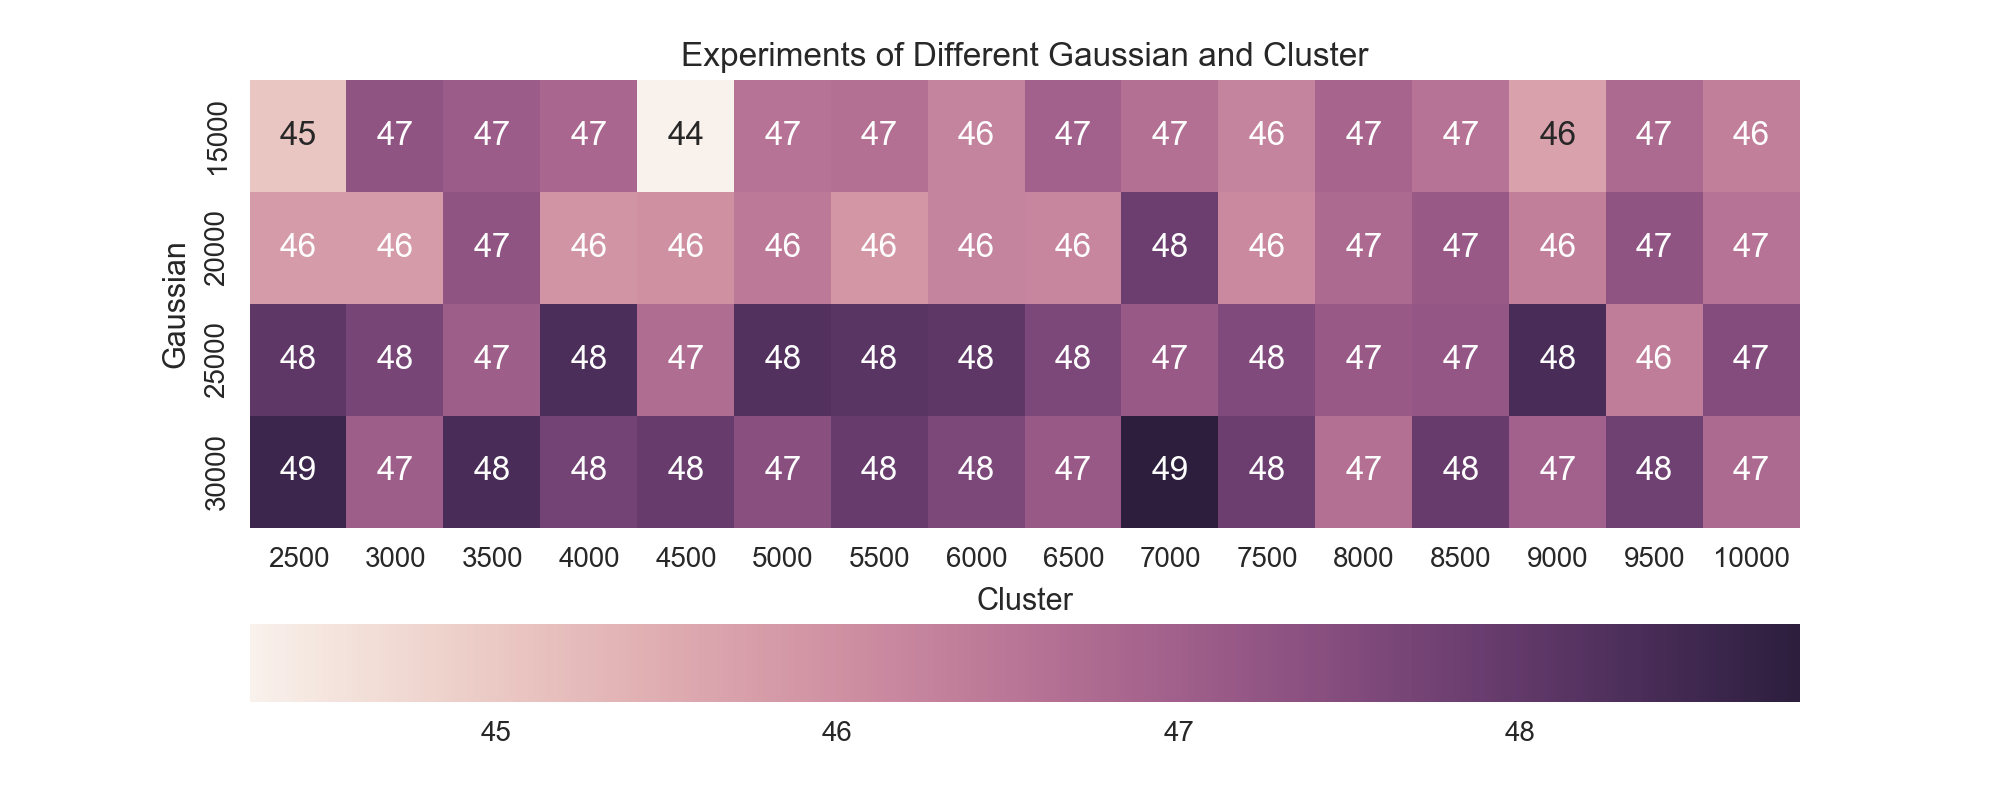
\includegraphics[width=3.2in]{result1_wer_heatmap.png} 
Figure 3.1: The Bitmap of WER against numbers of clusters and Gaussian mixture components. 
\end{center}

We can see that the lowest WER occurs when number of cluster is 4500 and number of Gaussian mixture components is 15000.

However, through this plot, we cannot investigate the evolution of WER towards clusters and Gaussian. So, we exponentially search the results with the number of cluster from 1000 to 3000 with the step of 500. And we search Gaussian based on the exponential of cluster. For example, if we set the number of cluster to 1000, we will search Gaussian of 1000,2000,4000,8000,16000...(for the exponential of cluster). Below is the plot of the evolution.

\begin{center}
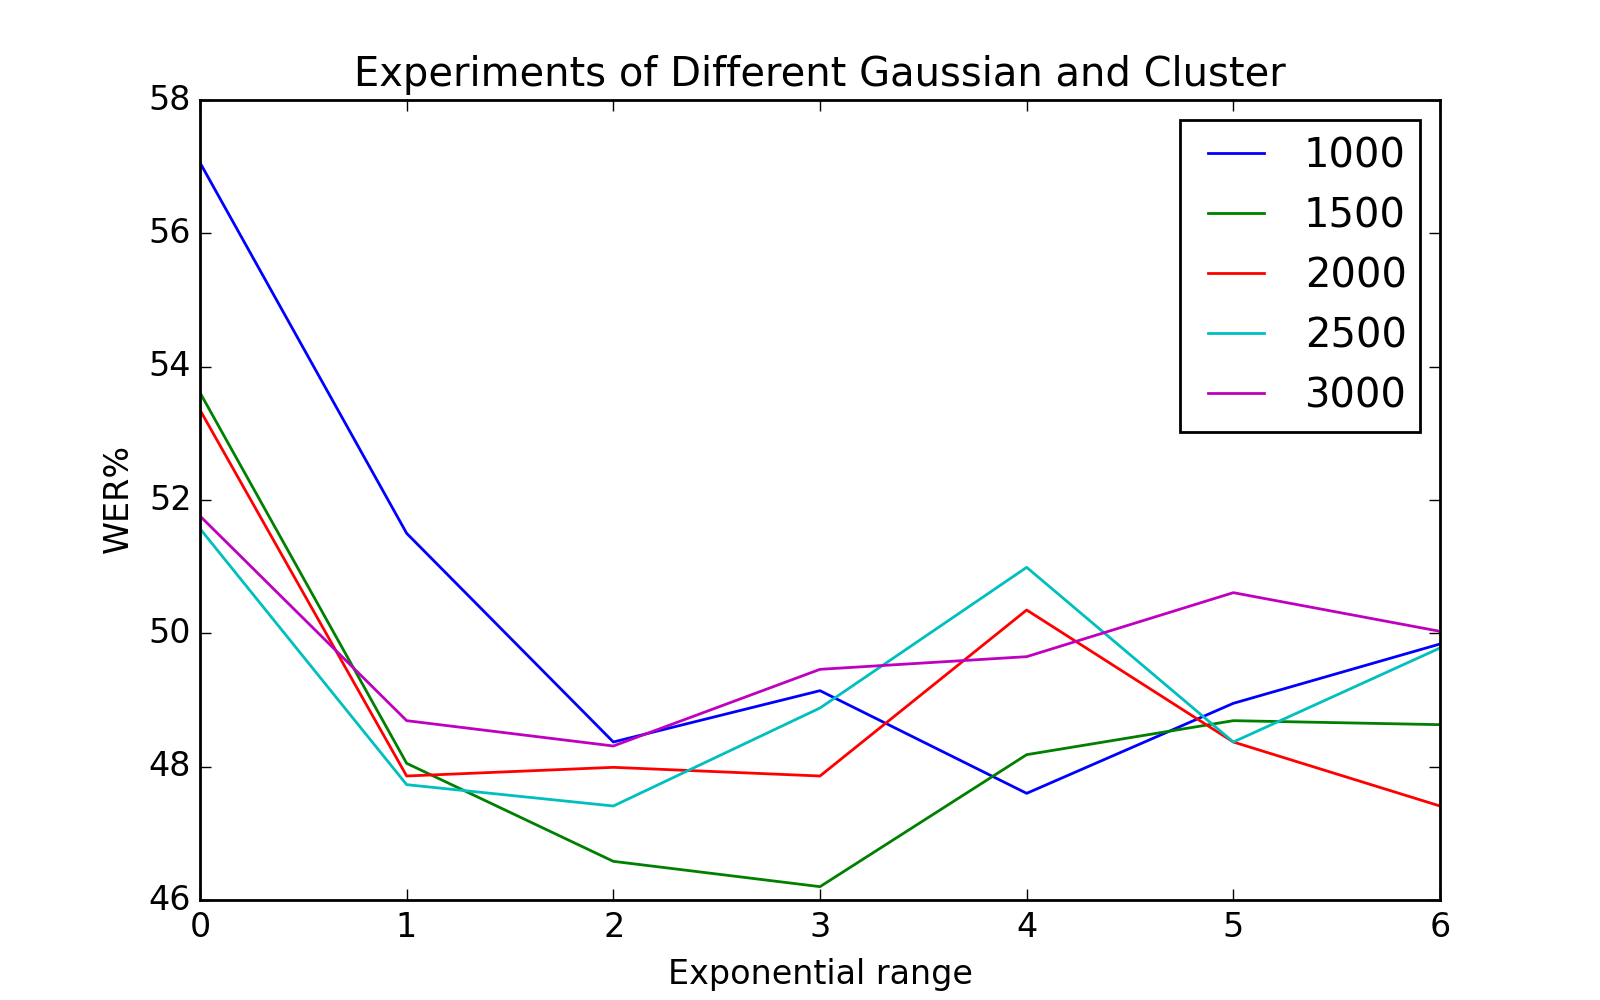
\includegraphics[width=3in]{result1_tri_small.png} 
Figure 3.2: The evolution of WER towards cluster and Gaussian 
\end{center}

\subsubsection{Conclusion and Discussion}

From the figure 3.1, it's difficult to find a general relationship among cluster and Gaussian towards WER. So, we changed our searching strategy to fix the number of cluster and search Gaussian exponentially. And surprisingly, the evolution becomes very clear. With the increase of Gaussian, the WER decreases and when the number of Gaussian exceed $2^3$ times of the number of cluster, the WER starts fluctuating. So, from our experiment, we could conclude that the good result could be obtained when the Gaussian is $2^2$ to $2^3$ times larger than cluster.

In addition, by comparing with the monophone model result, we could easily find that the triphone model could give better result since monophone model is a context independent method. By contrast, the triphone model considers the left and right possible phones to enhance the relevance of different phones.

For further work, we will use the triphone model we get in this experiment to see if we could improve it.

\section{Adaptive Training}
\subsection{Gender Dependent System}
\subsubsection{Purpose}
The aim of this task is to develop gender dependent acoustic models and make the recognition.
\subsubsection{Implementation}
To train a gender dependent model, we manually split the data into two part: female subset and male subset. We implement this by writing a python file to split the original data file.(the python file is stored in $my-local/split\_data\_gender.py$)

In the training part, we train monophone model for subsets first to get the monophone alignment. Then, we use the alignment to train triphone model. The detailed implementation could be found in $exp\_t3.1.sh$ script.

scripts: \textbf{\\ \indent exp\_t3.1.sh}

\subsubsection{Experiment and Result}
We split the original dataset into two parts. The information of two parts is shown in below table.

\begin{center}
Table 4.1: Gender dependent subsets

\begin{tabular}{c c}
\toprule
Gender & Number of data  \\
\midrule
Female & 524 \\
Male & 1041 \\
\bottomrule
\end{tabular}
\end{center}

From the table, we could see that there are 524 utterances in female subset and 1041 in male subset.

\begin{center}
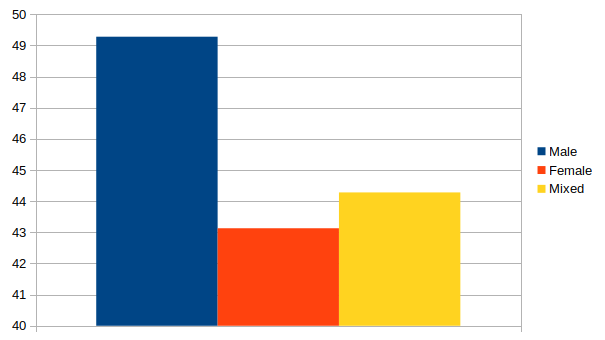
\includegraphics[width=3in]{plot.png} % need to change
Figure 4: WER of gender dependent acoustic model and original model.
\end{center}

We can see the gender dependent acoustic model improves the WER. The WER of female acoustic  recognition is 43.13\% and the WER of male acoustic recognition is 49.38\%. Comparing with the original baseline model(44.28\%) we obtained in task 2, the female recognition is better while the male recognition is worse.

\subsubsection{Conclusion and Discussion}
Generally, a gender dependent system could get a very good result compared with the original system for the reason that the speaker characteristics arise from systematic variations such as those arising from speaker age and accent will cause difficulty in recognition. And the gender dependent system could avoid this kind of problem.

However, our result doesn't show very good result(experiment gets worse result on male subset and better result on female subset). With discussion, we think this may relate to the quantity of training data. Since after splitting the data, we training data for each subset become less. Less training data will make the model not fully trained. So, to get a better result, we need to do further search to see if there exist a better result.

\subsection{Feature Transformation and Adaptive Training}
\subsubsection{Purpose}
In this section, we want to investigate one feature transformation method and one adaptive training method. For the feature transformation, we use Vtln feature to normalize the data. And for the adaptive training method, we try fMLLR method to see if it could improve the model.

\subsubsection{Implementation}
For the implementation part of vtln feature, we use $train_lvtln.sh$ to replace $train_deltas.sh$ and set the number of cluster to 4500, the number of Gaussian to 15000. Also, the decode process should be changed to $decode_lvtln.sh$.(For the detailed experiment script, see $exp_t3.2.sh$)

For the implementation part of fMLLR method, the $train_sat.sh$ script should be used to replace $train_deltas.sh$ and correspondingly, the decode script should be changed to $decode_fmllr.sh$.(For the detailed experiment script, see $exp_t3.2.sh$)

scripts: \textbf{\\ \indent exp\_t3.1.sh  \\ \indent exp\_t3.2.sh}

\subsubsection{Experiment and Result}
We run two scripts introduced above and the results are shown in below table.

\begin{center}
Table 4.2: WER of feature transformation method and adaptive training method

\begin{tabular}{c c}
\toprule
Method & WER\%  \\
\midrule
None & 44.23 \\
Vtln & 44.15 \\
fMLLR & 39.94 \\
\bottomrule
\end{tabular}
\end{center}

The table shows that both Vtln and fMLLR could provide better result though Vtln only achieves a little bit improvement.

\subsubsection{Conclusion and Discussion} 

Vocal tract length normalisation(VTLN) is to linearly scale the filter bank centre frequencies within the front-end feature extractor to approximate a canonical formant frequency scaling.(Lee,1996) The advantage of this approach is that the optimal transformation parameters can be determined from the auxiliary function in a single pass over the data. So, the vtln feature could effectively adapt to different gender and accent.

Maximum likelihood linear regression(MLLR) is a set of linear transforms are used to map an existing model set into a new adapted model set such that the likelihood of the adaptation data is maximised. From the experiment, we could investigate that the MLLR is generally very robust, which provides the best result.

With limited computational resources, we only compared two different method with the baseline model we got in task 2. Both of these methods give better result with the same condition. However, since we don't do further research on these two methods, it's hard to say which one is better than another one.

\section{Conclusion}

In this experiment, we did different experiments on monophone model and triphone model. In the experiments of monophone model, we obtained the best result with the number of Gaussian of 9700. And then, we did experiments to see if different features, dynamic features and CMN/CVN could improve the performance. Both dynamic features and CMN/CVN could give better result and the feature that gives the best result is MFCCs.

The experiments of triphone model indicates that triphone model could get better result comparing with the monophone model and we reach the best result when the number of cluster is 4500 and the number of Gaussian is 15000.

The experiments of gender dependent system shows that such system may not always improve the performance though it gets better result in female subset. Finally, by trying vtln and MLLR, we find that feature transformation methods and adaptive training methods could significantly improve the performance. 

\begin{thebibliography}{9}

\bibitem{gy2007}
  G\&Y: MJF Gales and SJ Young (2007).
  \emph{The Application of Hidden Markov Models in Speech Recognition},
  Foundations and Trends in Signal Processing,
  1 (3), 195-304.
\bibitem{rh2010}
  R\&H:S Renals and T Hain (2010).
  \emph{Speech Recognition, in Computational Linguistics and Natural Language Processing Handbook},
  A Clark, C Fox and S Lappin (eds.),
  Blackwells, chapter 12, 299-332.
\bibitem{wp2001}
  Woodland, Phil C.
  \emph{"Speaker adaptation for continuous density HMMs: A review."},
  ISCA Tutorial and Research Workshop (ITRW) on Adaptation Methods for Speech Recognition. 2001. 
\bibitem{LL1996} 
   L. Lee and R. C. Rose, 
   \emph{“Speaker normalisation using efficient frequency warping procedures”},
   in Proceedings of ICASSP, Atlanta, 1996.

\end{thebibliography}

\end{multicols*}
\end{document}